\documentclass[12pt, a4paper, openright, draft]{memoir}
\usepackage{fontspec}
\let\ordinal\relax %! Fixes \ordinal conflict with memoir
\usepackage[us]{datetime}
\newdate{startdate}{15}{3}{2020}
\usepackage{paracol}

\usepackage{expex, tikzvowel, phonrule}


\usetikzlibrary{fit}
\newdimen\contourraise
\newdimen\contourspacetokenwidth
\newcount\lasttokennumber
\newcount\currenttokennumber
\newcount\contourmarkcount
\newcount\contourtokenunderlinestate
\newbox\contourbox

\tikzset{
  tight fit/.style={
      inner sep=0pt,
      outer sep=0pt,
    },
  %
  %
  % How far above the reference anchor of the text,
  contour raise/.code=\pgfmathsetlength\contourraise{#1},
  contour reference anchor/.store in=\contourreferenceanchor,
  contour reference anchor=base east,
  % The `scale' for the values in the contour height specification
  contour scale/.store in=\contourscale,
  contour scale=3pt,
  % The prefix for the contour marks.
  contour mark prefix/.store in=\contourmarkprefix,
  contour mark prefix=contour,
  % The style for the contour path
  contour/.style={
      draw,
      rounded corners=1ex,
    },
  % The style for the token nodes
  every contour token/.style={
      anchor=base west,
      inner sep=0pt,
    },
  contour underline/.style={
      draw
    },
  % The character to insert a mark (use with care)
  contour mark character/.store in=\contourmarkchar,
  contour mark character=|,
  % Want to change the code for contour marks? Use this key.
  contour mark code/.store in=\contourmarkcode,
  % Want to change the code for tokens? Use this key.
  contour token code/.store in=\contourtokencode,
  % Want to change the code for drawing the contour? Use this  key.
  contour code/.store in=\contourcode,
  %
  % Default stuff
  contour mark code={%
      \coordinate (\contourmarkprefix-\the\contourmarkcount)
      at ([yshift=\contourraise, y=\contourscale,
        shift={(0,\currentcontourheight)}]token-\the\currenttokennumber.\contourreferenceanchor);
    },
  contour token code={%
      \node [every contour token/.try] at
      (token-\the\lasttokennumber.base east)
      (token-\the\currenttokennumber) {\token};
    },
  contour code={
      \draw [contour] (\contourmarkprefix-1)
      \foreach \y in {2,...,\the\contourmarkcount}{ --
          (\contourmarkprefix-\y) };
    },
  %
  % Don't draw the contour.
  tokens only/.style={
      contour code={}
    },
  %
  % Only draw the contour (but the space is still used for the tokens)
  contour only/.style={
      every contour token/.append style={
          execute at begin node={\setbox\contourbox=\hbox\bgroup},
          execute at end node=\egroup\phantom{\box\contourbox}%
        },
      underline/.style={
          draw=none
        }
    },
  %
  % Make tokens follow the contour marks.
  tokens follow contour/.style={
      tokens only,
      contour token code={%
          \node [every contour token/.try, y=\contourscale] at
          (token-\the\lasttokennumber.base east |-
          0,\currentcontourheight)
          (token-\the\currenttokennumber) {\token};
        },
    },
  % What style to use when drawing underline
  underline/.style={
      draw
    },
  % The underline is drawn along the south side of a node which
  % takes this style.
  underline token/.style={
      inner ysep=1pt
    },
  % When grouping tokens (e.g., for putting box around)
  % this style is applied to a node that is fitted around the group
  token group/.style={
      inner xsep=1pt,
      inner ysep=2pt,
      rounded corners=2pt
    },
  % Draw boxes around tokens groups.
  box tokens/.style={
      token group/.append style={
          draw
        }
    },
  % Change the width of the spaces.
  space token width/.code=\pgfmathsetlength\contourspacetokenwidth{#1},
  space token width=0.125cm
}

\makeatletter

\def\at@{@}

\newcommand\contour[2][]{%
  \begin{scope}[#1]
    \coordinate (token-0);
    \currenttokennumber=0\relax%
    \lasttokennumber=0\relax%
    \contourmarkcount=0\relax%
    \def\lastcontourheight{0}%
    \contourtokenunderlinestate=0\relax%
    \@contour#2@%
    }

    % Must check for a spaces
    \def\@contour{\futurelet\@token\@checkforspace}

    \def\@uscore{_}
    \def\@checkforspace{%
      \ifx\@token\@sptoken%
        \let\@next=\@replacespace%
      \else%
        \if\@token\contourmarkchar%
          \let\@next=\@contour@insertmark
        \else%
          \if\@token\@uscore
            \let\@next=\@contourtoggleunderline%
          \else%
            \let\@next=\@@contour%
          \fi%
        \fi%
      \fi%
      \@next%
    }

    \def\@contourtoggleunderline#1{%
      \advance\contourtokenunderlinestate by1\relax
      \ifnum\contourtokenunderlinestate>3\relax%
        \contourtokenunderlinestate=0\relax%
      \fi%
      \@contour%
    }

    \def\@contour@insertmark{%
      \afterassignment\@@contour@insertmark\let\@token=%
    }

    \def\@@contour@insertmark{%
      \futurelet\@token\@@@contour@insertmark}%

    \def\@@@contour@insertmark{%
    \if\@token[%
      \let\@next=\@@@@contour@insertmark%
    \else%
      \let\currentcontourheight=\lastcontourheight%
      \let\@next=\@@@@@contour@insertmark%
    \fi%
    \@next%
    }

    \def\@@@@contour@insertmark[#1]{%
      \def\@tmp{#1}%
      \ifx\@tmp\@empty%
        \let\currentcontourheight=\lastcontourheight%
      \else%
        \def\currentcontourheight{#1}%
      \fi%
      \@@@@@contour@insertmark}

    \def\@@@@@contour@insertmark{%
      \advance\contourmarkcount by1\relax%
      % Code for inserting mark
      \contourmarkcode%
      \let\lastcontourheight=\currentcontourheight%
      \@contour}

    \def\contourspacetoken{{\hbox to \contourspacetokenwidth{\hfill}}}

    \def\@replacespace#1{%
      \@contour\contourspacetoken#1%
    }

    \def\@@contour#1{%
      \def\@token{#1}%
      \if\@token\at@%
        \@contourdounderline%
        \pgfutil@ifundefined{pgf@sh@ns@tokengroup}{}{%
          \node [tight fit, fit={(tokengroup)}, token group/.try] {};
          \global\let\pgf@sh@ns@tokengroup=\relax%
        }%
        \let\@next=\@@@contour%
      \else%
        \lasttokennumber=\currenttokennumber%
        \advance\currenttokennumber by1%
        \let\token=\@token%
        % Code for typesetting token
        \contourtokencode%
        % Manage underline state
        \@contourdounderline%
        \def\@@token{\contourspacetoken}%
        \ifx\@token\@@token%
          \pgfutil@ifundefined{pgf@sh@ns@tokengroup}{}{%
            \pgfutil@ifundefined{pgf@sh@ns@underline}{}{%
              \node [tight fit, fit={(tokengroup) (underline)}]
              (tokengroup)
              {};}%
            \node [tight fit, fit={(tokengroup)}, token group/.try] {};
            \global\let\pgf@sh@ns@tokengroup=\relax%
          }%
        \else
          \pgfutil@ifundefined{pgf@sh@ns@tokengroup}{%
            \node [tight fit,
              fit={(token-\the\currenttokennumber)}]
            (tokengroup) {};
          }{%
            \node [tight fit,
              fit={(token-\the\currenttokennumber)
                  (tokengroup)}]
            (tokengroup){};
          }%
        \fi%
        \let\@next=\@contour
        %
      \fi%
      \@next%
    }

    \def\@contourdounderline{%
      \ifcase\contourtokenunderlinestate%
      \or
        \node [tight fit, fit={(token-\the\currenttokennumber)}]
        (underline) {};
        \contourtokenunderlinestate=2\relax%
      \or%
        \node [tight fit,fit={(token-\the\currenttokennumber) (underline)}]
        (underline) {};
      \or%
        \node [tight fit, fit={(underline)}, underline token/.try]
        (underline) {};
        \draw [underline/.try]
        (underline.south west) -- (underline.south east);
        \pgfutil@ifundefined{pgf@sh@ns@tokengroup}{}{%
          \node [tight fit, fit={(tokengroup) (underline)}]
          (tokengroup) {};%
          \node [tight fit, fit={(tokengroup)}, token group/.try] {};
          \global\let\pgf@sh@ns@tokengroup=\relax%
          \global\let\pgf@sh@ns@underline=\relax%
        }
        \contourtokenunderlinestate=0\relax
      \fi%
    }
    \def\@@@contour{%
    \ifnum\contourmarkcount>1
      % Code for drawing contour
      \contourcode%
    \fi%
  \end{scope}%
}

\makeatother


\usepackage[hidelinks]{hyperref}
\hypersetup{linktoc=all}

\titlingpageend{\clearforchapter}{\clearforchapter} %! Titlingpage/openany fix for blank page
\pagestyle{ruled}
\makeoddfoot{plain}{}{}{\thepage}
\makeevenfoot{plain}{\thepage}{}{}
\copypagestyle{title}{empty}

\setmainfont{Libertinus Serif}

\setlength{\parindent}{0pt}
\nonzeroparskip

\lingset{
  glstyle=nlevel,
  belowglpreambleskip={-.5\parskip},
  aboveglftskip={-.5\parskip},
  exskip={0pt},
  glneveryline={,\it,\nogloss}
}

% Doc specific stuff
\newcommand{\langword}[1]{\textit{#1}}
\newcommand{\langname}{Ahale}

\newcommand{\pronounced}[1]{\vskip-0.5\parskip[#1]}


\begin{document}
\title{\langname : A Complete Reference}
\author{Pancake}
\date{\DTMusedate{startdate} - \DTMtoday}
\frontmatter
\begin{titlingpage}
  \maketitle
\end{titlingpage}

\begin{KeepFromToc}
  \tableofcontents
\end{KeepFromToc}
\mainmatter

\chapter{Introduction}\label{ch:introduction}
\section{Conventions}\label{sec:conventions}
In this document, italic text will be used for native \langname\ words, unless enclosed in angle brackets (\nativetext{ahale} or \orthotext{ahale}, but never \orthotext{\nativetext{ahale}}).
\aside{This aside is from an internal perspective. It may discuss things such as word choice, or the cultural significance of phrases.}
\aside{\fleuron\ This aside is from an external perspective. It may discuss design choices or other such self-imposed challenges.}
The former is found mostly in running prose, and the latter in places where a word is being used as a more self-contained example, or simply if orthography is of particular interest.

\phomtext{forward slashes} are used for phonemic transcriptions, while \phontext{square brackets} are used for phonetic transcriptions.

When words are exemplified within prose, they are often followed by a short translation. These will be written surrounded by \transtext{single quotes}.

Notable terms will be written \notabletext{like this.}

``Double quotes'' are used for non-standard, ironic, or otherwise deviant use of terms.

\subsection{Document Structure}
Most of the content contained within this grammar will be found in the main prose. However, footnotes along with margin notes will be used for tangential or, in the case of footnotes, explanatory details about particular terms.

Margin notes will be reserved for explanation of decisions made in the various translations, or in the usage details of a specific construction.
In the case of notes from an external perspective, being preceded by a fleuron (\fleuron).

\subsection{Glossing}\label{sec:conventions-gloss}
Glosses are generally constructed as follows:

\begin{example}
  \lect Dialect
  \preamble Romanization (undelimited)
  \pronunciation pronunciation
  \gloss
    morphemic & morphemic \\
    transcription & transcription \\
    (object language) & (metalanguage) \\
  \tr Translation
  \source Source
\end{example}

\section{History}\label{sec:history}
\subsection{Internal}\label{sec:hist-int}

\subsection{External}\label{sec:hist-ext}
\langname\ is the spiritual successor to my first conlang, Wei. As with many first attempts at conlanging, I consider Wei to be poorly made, and even more poorly described. Because of this, I consider \langname\ a successor only on account of my initial intentions.

Wei was very anglocentric, only a few steps away from a full relex, if even that. After I pronounced Wei abandoned in September 2019, I took a long break, and used that time to learn more about linguistics so that when I returned, I felt at least somewhat more prepared to make something I would be proud of.

When I began work on \langname , I wanted to stray as far away from my original mistakes as I could do comfortably. With that in mind, I outlined just a few goals for myself:

\begin{itemize}
  \item A morphosyntactic alignment other than nominative-accusative
  \item A minimalistic phonology which I would still be comfortable pronouncing
  \item Relatively free word order
  \item Some degree of non-concatenative morphology
  \item Thorough documentation, with many examples to explain nuances in translation (another goal of mine)
  \item Generally be interesting, fun, and fulfilling to work on
\end{itemize}

As the documentation currently stands, I feel I have achieved, and continue to work to achieve many of these goals. Depth of documentation, and nuance of lexical entries is something I'm still working on. Throughout the various iterations of this document, I hope that I can continue to improve on these areas to an even greater extent than I have at the time of writing this section.\footnotemark

\footnotetext{Last updated \DTMdisplaydate{2021}{1}{31}{-1}
}
\subsubsection{Typological Details}
While I don't find typology a terribly informative tool in regards to how language \textit{actually} functions, it can serve as an overview of concepts which will be encountered. As such, here's (another) short list of bullet points:

\begin{itemize}
  \item Utilizing a direct-inverse verbal system (resulting in a syntactically \textit{hierarchical} alignment)
  \item Ergative-absolutive morphology
  \item Strong pro-drop tendencies
  \item (A lot of) reduplication
  \item Use of verb serialization
\end{itemize}

In essence, the things which I find interesting.

\part{Phonology}\label{prt:phonology}
\chapter{Segmental Phonology}\label{ch:seg-phono}
\section{Inventory}\label{sec:phono-inv}

\begin{table}[ht]
  \centering
  \begin{tabular}{*{7}{c}}
    \toprule
    & Labial & Alveolar & Velar & Glottal \\\midrule
    Plosive   & p      & t        & k     & ʔ       \\
    Nasal     & m      & n        &       &         \\
    Fricative & ɸ      & s        & x     & h       \\
    Sonorant  & w      & l        &       &         \\
    \bottomrule
  \end{tabular}
  \caption{Consonant Inventory}
  \label{table:consonants}
\end{table}

\aside{\fleuron \phontext{e} is an allophone of \phomtext{ə}, rather than a phoneme unto itself as it may first appear, (see \textsc{rel} and \textsc{assoc} \nativetext{ʔe})
}

\begin{figure}[ht]
  \centering
  \begin{vowel}
    \vpoint{0}{0}{i}
    \vpoint{0}{2}{u}
    \vpoint{1.5}{1}{ə}
    \vpoint{3}{1}{a}
    \varrow{a}{u}
    \varrow{a}{i}
  \end{vowel}
  \caption{Phonemic Vowel Inventory}
  \label{table:vowel_phonemes}
\end{figure}

Diphthongs consisting of \phomtext{ə} + high vowel can be observed in a few words, however these diphthongs are prone to collapse. In all but the most conservative of dialects, these are realized as \phomtext{əi əu} \phontext{e o}.

\vfill %! This is not smart don't do this
\section{Stress}
\subsection{Assignment}
Stress is generally assigned to the initial syllable of a root. However, \phomtext{ə} generally will not recieve stress at this stage and move to the second syllable (even if this is also a schwa).

A subset of affixes (including, but not limited to those which utilize reduplication) are considered ``weak'', in that, like schwa, they repel stress.

Such morphemes will be marked with a comma in morphemic transcription, rather than the usual period used at syllable boundaries. Thus \morphtext{ʔə,} refers to a morpheme \phomtext{ʔə} which repels stress.

\subsection{Realization}
Under most circumstances, lexical stress is realized as a slight rise in pitch on the affected syllable, which then gradually falls back to ``standard'' pitch across the remaining part of the word. Because stress is very strongly initial, this means that generally, pitch will fall gradually across words and phrases.

This is of course also affected by phrase- and sentence-level prosody, which will be discussed in \Cref{ch:suprasegmental-phonology}.

\section{Allophony}
This section will be structured a bit differently from the others encountered thus far. Because allophony and diachronic processes in general occur in a particular order, Sectioning will be used to separate larger processes from those more easily described in standard notation.

While this document will cover some dialectical differences, examples given which include phonetic information Will be in reference to a standard dialect, \textbf{Literary Standard \langname}, Which will be abbreviated LSA

The ordering of rules will begin below, and these larger processes will be contained within subsections which will be referenced in the list.

\begin{enumerate}
  \item {
    Stressed \phomtext{ə} becomes \phontext{e}

    \phon{ə\phonfeat{+stress}}{e}
    }
  \item \titleref{sec:allophony-lengthening}
  \item {
    \phontext{ə} is elided between homorganic consonants

    \phonc{ə}{Ø}{\phonfeat{αcplace} \phold \phonfeat{αcplace}}
    }
    \item {
      \phontext{n} + plosive clusters cause place assimilation of the nasal

      \phonc{\phonfeat{+nasal}}{\phonfeat{αcplace}}{\phold \phonfeat{-cont}}
  }
    \item {
      Nasal + plosive clusters assimilate

      \phonc{\phonfeat{-cont}}{\phonfeat{+nasal}}{\phonfeat{+nasal} \phold}
  }

  \item {
      Unstressed final vowels are elided

      \phonc{V\phonfeat{-stress}}{Ø}{\phold \$}
  }
  % \aside{\fleuron\ If I'm being completely honest, I have no idea why the process of affrication is done with +delayed release. I'm simply following the conventions as outlined by \url{http://www.artoflanguageinvention.com/papers/features.pdf}}
  % \item {
  %     Word final geminated plosives are affricated

  %     \phonc{C\phonfeat{-cont \\ +long}}{C\phonfeat{+del release\footnotemark \\ -long}}{\phold \$}
  % }

\end{enumerate}

\subsection{Prosodic Lengthening}\label{sec:allophony-lengthening}
In some situations, syllable shape can cause gemination of the surrounding syllables--- prosodic lengthening, if you will, to allow for more consistent syllable-timing. The most notable of these situations is when a CV syllable, where C is a plosive, comes after a CVV sequence\footnotemark\ beginning in a non-plosive consonant.

\footnotetext{This is described as a CVV \textit{sequence} rather than a CVV syllable, because this process is not dependent on \phontext{VV} being a true diphthong. This can be seen in the first example, where \phontext{ua} Is not a diphthong but still triggers this change.}

Thus, pairs such as the following hypothetical forms may emerge:
\begin{itemize}
  \item \phomtext{suaki} \phontext{ˈsu.a.kːi} and \phomtext{suki} \phontext{ˈsu.ki}
  \item \phomtext{maipi} \phontext{ˈmai.pːi} and \phomtext{mapi} \phontext{ˈma.pi}
  \item \phomtext{iwəiku} \phontext{ˈi.we.kːu}\footnotemark\ and \phomtext{iwəku} \phontext{ˈi.wə.ku}
\end{itemize}

\footnotetext{This more aggressive simplification of diphthongs may give the appearance that plosives may geminate without an apparent trigger. Of course, this only applies to dialects which do not preserve the original diphthongs.}

\aside{\fleuron\ While moraic analysis of this process is not typical, one might suppose that this process is triggered by a heavy syllable followed by a light one, and that CVV is heavy, while VV is not.}
One thing of note is that the onset of the CVV syllable is mandatory to trigger this process. Observe the following hypothetical forms, Which do not undergo this change due to their VVCV shape:
\begin{itemize}
  \item \phomtext{auku} \phontext{ˈau.ku}
  \item \phomtext{aiʔi} \phontext{ˈai.ʔi}
  \item \phomtext{euti} \phontext{ˈo.ti}
\end{itemize}


% \chapter{Suprasegmental Phonology}\label{ch:suprasegmental-phonology}
On

\backmatter
% bibliography, glossary and index would go here.
\chapter{Passages}
\begin{comment}

  \begin{verbatim}
    heya <<vendor>>
    <vendor> siʔe
    Bright <vendor>. (This is a bit formal but not much since <vendor> is working)

  oi Teɸinu, how's it going?
  mili hasi <customer>?
  "You are as you should? (certain; in interrogatives this primes expectations but anything less than mili is
  rude unless already engaged in convo)"

  well, I heard there's about to be a storm
  wa me kana, pa suaki ɸai hipese
  AFF I heard this, then [strong wind won't be contained] (anymore) // ɸai is being used as a subordinating
  conjunction here

  yeah, seems like one of the big ones -- you looking for something?
  wa suaki, taʔe ki -- kisuɸi auku?
  [ AFF wind_blow ] prox-assoc (resumptive ta because verbs cannot be the head of a typical relative clause)
  big -- WONDERING look(2sg)

  ye nah I was thinking <<bad idea>> but I'm not sure now—
  <<papaya>>?
  meme imipi iniha ta <<paʔawa>> lu, kini ʔike ɸai meme
  1sg.erg think-pst.ipfv give-pst.ipfv prox papaya obv, know neg 1sg.erg

  how bout some yams instead, eh?
  Meme leha upe...
  erg-1sg have.npst.ipfv yam

  yams?
  lelewine?
  uncert

  yeah, good stuff
  wa, luʔe kate
  AFF OBV-ASSOC good

  that's... alright, yams, how many dyou have?
  kiniʔe kate... atai leha tutu upe?
  this-ASSOC good | number have 2sg yam

  lemmesee... <<counts>> I've got <<number>>, how's four? couple extra in case it gets
  wild
  me auku --- ai, ni, ku,... niheu upe, ha kiniʔe kate pa ilaʔe xaku
  1sg see --- one two three ... twenty yam | four this good now gift [from] pain

  mhm, sounds alright - that's <<sum>>, yeah?
  wa, kiniʔe kate - nataʔe kisuɸi ki
  aye, this is nice - that's a lot (kinda certain)

  ye, nah, since there's a storm I'll let you have them for <<smaller sum>>
  wa. suaki ɸai hipese pa upeʔe tele

  if you insist, I spose I can always—
  lelewine paki, mai mapi

  I'm gonna pack away soon, so just-
  pa lau---

  yeah ok-
  wa-

  -just, just take them
  tutu niha ta

  -free?
  mapiʔe ila?
  whole-assoc gift

  you'll pay me later, go, take ca-
  nihasi ila lu me, Tu(ʔe si).

  -ah thanks-
  ɸawa

  -care-
  (ʔe si)

  ye alright, see you
  taʔe kate, iaukusi alete aukusi

  bye!
  meme hasi ta
  I am as I should

  mumbling yams, yams... shit, how many do I have left now
  Pa upe upe, atai leha meme upe?
  \end{verbatim}


  \ex
  \begin{tikzpicture}
    \contour[contour raise=0.5cm]
    {|[2]Nalexu|[2] siʔe|[6]}
  \end{tikzpicture}

  \begingl
  Nalexu[\textsc{name}]
  si-ʔe[brightness\textsc{-assoc}]
  \glft \transtext{Hey Nalexu!} \\ \hspace*{1em}\textsc{lit.} \transtext{Bright Nalexu!}
  \endgl
  \xe
  {
    \color{red}
    \ex

    \begin{tikzpicture}
      \contour[contour raise=0.5cm]
      {|[3]Mili |[4]ha|[2]si |[1]Teɸi|[2]nu?}
    \end{tikzpicture}

    \begingl
    mili[\textsc{certain}]
    hasi[continue\textsc{[q]}]
    Teɸinu[\textsc{name}]
    \glft \transtext{How are you doing, Teɸinu?} \\ \hspace*{1em}\textsc{lit.} \transtext{You are as you should be, Teɸinu?}
    \endgl
    \xe
    }

    In interrogatives, certainty particles used this way prime expectations of the answer, but anything less than \nativetext{mili} is rude unless already engaged in conversation where \nativetext{mili} is deemed unfit.

    \ex

    \begin{tikzpicture}
      \contour[contour raise=0.5cm]
      {|[2]Wa me |[6]kana|[2] pa|[5] |[2]suaki ɸai|[1] hipese|[2]}
    \end{tikzpicture}

    \begingl
    wa[\textsc{aff}]
    me[\textsc{1sg}]
    kana[hear]
    pa[now]
    suaki[wind\_blow]
    ɸai[\textsc{conj}]
    hipese[contain]
    \glft \transtext{`I heard there's about to be a storm?} \\ \hspace*{1em}\textsc{lit.} \transtext{Well, I heard soon that the wind won't be contained.}
    \endgl
    \xe

    \nativetext{ɸai} is being used as a negative subordinating conjunction here.

    \ex
    {
      \color{red}
      \begin{tikzpicture}
        \contour[contour raise=0.5cm]
        {  |[2]wa |[6]suaki, |[3]taʔe ki|[2] -- |[4]kisuɸi |[2]auku?|[3]}
      \end{tikzpicture}

      \begingl
      wa[\textsc{aff}]
      suaki[wind\_blow]
      taʔe[\textsc{prox-assoc}]
      ki[big]
      kisuɸi[\textsc{wonder}]
      auku[see]
      \glft \transtext{Yeah, seems like one of the big ones -- you looking for something?}
      \endgl
      \xe}

      \ex


      \begin{tikzpicture}
        \contour[contour raise=0.5cm]
        {|[2]meme |[6]imipi|[3] iniha ta|[6] paʔawa lu, |[4]kini |[2]ʔike ɸai meme|[1]}
      \end{tikzpicture}

      \begingl
      me\textasciitilde me[\textsc{erg\textasciitilde 1sg}]
      i-mipi[\textsc{pst.ipfv-}think]
      i-niha[\textsc{pst.ipfv-}give]
      ta[\textsc{prox}]
      paʔawa[papaya]
      lu[\textsc{obv}]
      kini[\textsc{dem\_prox}]
      ʔike[know]
      ɸai[\textsc{neg}]
      me\textasciitilde me[\textsc{erg\textasciitilde 1sg}]
      \glft \transtext{Yeah, I was thinking papaya but I'm not sure now---}
      \endgl
      \xe
      {
        \color{red}
        \ex

        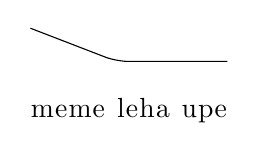
\begin{tikzpicture}
          \contour[contour raise=0.5cm]
          {|[6]meme |[2]leha upe|[2]}
        \end{tikzpicture}

        \begingl
        me\textasciitilde me[\textsc{erg\textasciitilde 1sg}]
        leha[have]
        upe[yam]
        \glft \transtext{Have some yams instead, eh?}
        \endgl
        \xe
        }
        \ex

        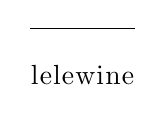
\begin{tikzpicture}
    \contour[contour raise=0.5cm]
    {|[2]lelewine|[2]}
  \end{tikzpicture}

  \begingl
  lelewine\textasciitilde\textasciitilde[\textsc{uncert}]
  \glft \transtext{Yams?}
  \endgl
  \xe
  \pagebreak
  {
    \color{red}
    \ex

    \begin{tikzpicture}
      \contour[contour raise=0.5cm]
      {|[2]wa |[5]luʔe |[3]kate|[2]}
    \end{tikzpicture}

    \begingl
    wa[\textsc{aff}]
    lu-ʔe[\textsc{obv-assoc}]
    kate[goodness]
    \glft \transtext{Yeah, good stuff.}
    \endgl
    \xe
    }
    \ex

    \begin{tikzpicture}
      \contour[contour raise=0.5cm]
      {|[4]luʔe kate\textasciitilde\textasciitilde|[2] |[7]atai leha tutu |[2]upe|[4]}
    \end{tikzpicture}

    \begingl
    kini-ʔe[\textsc{dem\_prox-assoc}]
    kate[goodness]
    atai[number\textsc{[q]}]
    leha[have]
    tu\textasciitilde tu[\textsc{erg\textasciitilde 2sg}]
    upe[yam]
    \glft \transtext{That's... alright. Yams--- how many do you have?}
    \endgl
    \xe
    {
      \color{red}
      \ex

      \begin{tikzpicture}
        \contour[contour raise=0.5cm]
        {|[2]me au|[4]ku\textasciitilde\textasciitilde|[2] |[2]ai|[4], |[2]ni|[4], |[2]ku,... |[6]niheu |[2]upe,|[1] |[4]ha kiniʔe|[2] |[5]kate|[2] |[5]pa ilaʔe |[4]xaku|[2]}
      \end{tikzpicture}

      \begingl
      me[\textsc{1sg}]
      auku[see]
      ai[one]
      ni[two]
      ku[three]
      niheu[ten]
      upe[yam]
      ha[four]
      kini-ʔe[\textsc{dem\_prox-assoc}]
      kate[goodness]
      pa[now]
      ilaʔe[gift\textsc{-assoc}]
      xaku[pain]
      \glft \transtext{I'll check... 1, 2, 3--- I’ve got ten, how’s four? A bit extra if it gets wild.}
      \endgl
      \xe}
      % With \nativetext{pa} rather than a more uncertain construction, the implication is that the happening is inevitable.

      \ex
      \begin{tikzpicture}
        \contour[contour raise=0.5cm]
        {|[2]wa|[2], |[4]kiniʔe kate|[2] - |[5]nataʔe kisuɸi|[3] ki|[1]}

      \end{tikzpicture}



      \begingl
      wa[\textsc{aff}]
      kini-ʔe[\textsc{dem\_prox-assoc}]
      kate[goodness]
      nata-ʔe[\textsc{dem\_med-assoc}]
      kisuɸi[\textsc{cert}]
      ki[big]
      \glft \transtext{Aye, this is nice -- that's a lot.}
      \endgl
      \xe

      {
        \color{red}
        \ex

        \begin{tikzpicture}
          \contour[contour raise=0.5cm]
          {|[2]wa suaki|[3] ɸai|[1] hipese|[3] pa upeʔe te|[1]le|[3]}

        \end{tikzpicture}


        \begingl
        wa[aff]
        suaki[wind\_blow]
        ɸai[\textsc{conj}]
        hipese[contain]
        pa[now]
        upe-ʔe[yam\textsc{-assoc}]
        tele[part]
        \glft \transtext{Hmm, since there’s a storm I’ll let you have them for less.}
        \endgl
        \xe
        }
        \ex

        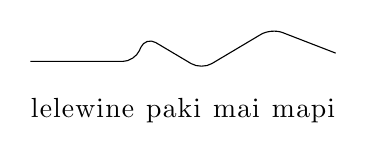
\begin{tikzpicture}
          \contour[contour raise=0.5cm]
          {|[2]lelewine|[2] |[5]paki|[1]  mai |[6]mapi|[3]}
        \end{tikzpicture}

        \begingl
        lelewine[\textsc{uncert}]
        paki[tell\_truth]
        mai[time]
        mapi[whole]
        \glft \transtext{If you insist, I'll always---}
        \endgl
        \xe

        {
          \color{red}
          \ex

          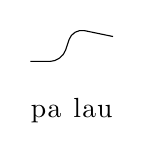
\begin{tikzpicture}
            \contour[contour raise=0.5cm]
            {|[2]pa|[2] |[6]lau|[5]}
          \end{tikzpicture}


          \begingl
          pa[now]
          lau[neaten]
          \glft \transtext{I'm gonna pack away soon, so just---}
          \endgl
          \xe
          }
          \ex

          
\begin{tikzpicture}
            \contour[contour raise=0.5cm]
            {|[4]wa|[6]}
          \end{tikzpicture}

          \begingl
          wa[\textsc{aff}]
          \glft \transtext{Yeah okay---}
          \endgl
          \xe
          {
            \color{red}
            \ex

            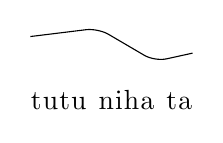
\begin{tikzpicture}
              \contour[contour raise=0.5cm]
              {|[4]tutu |[5]niha|[1] ta|[2]}
            \end{tikzpicture}

            \begingl
            tu\textasciitilde tu[\textsc{erg\textasciitilde 2sg}]
            niha[give]
            ta[\textsc{prox}]
            \glft \transtext{Just take them.}
            \endgl
            \xe
            }
            \ex

            \begin{tikzpicture}
              \contour[contour raise=0.5cm]
              {|[4]mapi|[4]ʔe |[2]ila|[3]}
            \end{tikzpicture}

            \begingl
            mapi-ʔe[whole\textsc{-assoc}]
            ila[gift]
            \glft \transtext{Free?}
            \endgl
            \xe
            {
              \color{red}
              \ex

              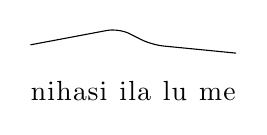
\begin{tikzpicture}
                \contour[contour raise=0.5cm]
                {|[2]nihasi |[4]ila|[2] lu me|[1]}
              \end{tikzpicture}


              \begingl
              niha-si[give\textsc{-inv}]
              ila[gift]
              lu[\textsc{obv}]
              me[\textsc{1sg}]
              \glft \transtext{You'll pay me later.}
              \endgl
              \xe}

              \ex

              \begin{tikzpicture}
                \contour[contour raise=0.5cm]
                {|[2]ɸawa|[1]si|[3]}
              \end{tikzpicture}


              \begingl
              ɸawa-si[thank\textsc{-inv}]
              \glft \transtext{Thank you!}
              \endgl
              \xe
              {
                \color{red}
                \ex

                \begin{tikzpicture}
                  \contour[contour raise=0.5cm]
                  {|[2]tu |[2]siʔe|[6]}
                \end{tikzpicture}

                \begingl
                tu[\textsc{2sg}]
                siʔe[brightness\textsc{-assoc}]
                \glft \transtext{Take care.}
                \endgl
                \xe
                }

                \ex

                \begin{tikzpicture}
                  \contour[contour raise=0.5cm]
                  {|[2]taʔe |[4]kate,|[2] |[5]iokusi|[3] a|[4]lete|[1] |[4]aukusi|[2]}
                \end{tikzpicture}

                \begingl
                ta-ʔe[\textsc{prox-assoc}]
                kate[good]
                i-auku-si[\textsc{pst.ipfv-}see\textsc{-inv}]
                alete[thus]
                auku-si[see\textsc{-inv}]
                \glft \transtext{Alright, see you later.}
                \endgl
                \xe


                {
                  \color{red}
                  \ex


                  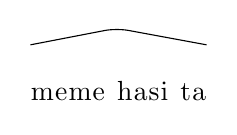
\begin{tikzpicture}
  \contour[contour raise=0.5cm]
  {|[2]meme |[4]hasi ta|[2]}
\end{tikzpicture}


\begingl
me\textasciitilde me[\textsc{erg\textasciitilde 1sg}]
hasi[continue]
ta[\textsc{prox}]
\glft \transtext{Goodbye.}
\endgl
\xe

\ex

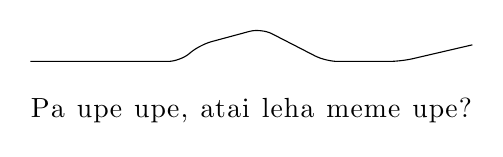
\begin{tikzpicture}
  \contour[contour raise=0.5cm]
  {|[2]Pa upe upe|[2], |[4]atai |[6]leha |[2]meme|[2] upe?|[4]}
\end{tikzpicture}

\begingl
pa[now]
upe[yam]
upe[yam]
atai[number]
leha[have\textsc{[q]}]
me\textasciitilde me[\textsc{erg\textasciitilde 1sg}]
upe[yam]
\glft \transtext{Yams, yams... shit, how many do I have left now?}
\endgl
\xe}
\end{comment}
\end{document}